\subsection*{\revise{NSC in Visual Cortex}}

\revise{Due to its roots in efficient-coding theories of natural image processing,
\ac{NSC} figures prominently in the vision neuroscience literature.}

\revise{For example, \ac{NMF}-based models were able to reconstruct
\emph{in vitro} neuronal spike trains from the salamander retina 
\cite{Onken2016,Liu2017}.
By combining spike-triggered average with \ac{NMF},
Liu and colleagues \cite{Liu2017} were able to identify the subunit layout
of retinal ganglion cells
(Fig.~\ref{fig:NMF|retina}).
Whereas modules were constrained to be have nonnegative elements,
stimuli were represented by their contrast values (i.e., their relative deviation from mean light intensity, which could be positive or negative).
The goal of their \ac{NMF} variant was then to seek weights and nonnegative modules
that minimize the difference, in a least-squares sense, between the spike-triggered
stimuli and the reconstruction.
Interestingly, the identified subunits corresponded to 
individual presynaptic bipolar cells,
as verified by multielectrode array recordings with simultaneous recordings from
individual bipolar cells through sharp microelectrodes \cite{Liu2017}.
This allowed the researchers to improve predictions about how ganglion cells respond
to natural stimuli, without the need to guess a specific model structure that may be constrained in terms of the size, shape, number, or nonlinearity of 
ganglion cell subunits.}

\begin{figure}[!b]
	\centering
	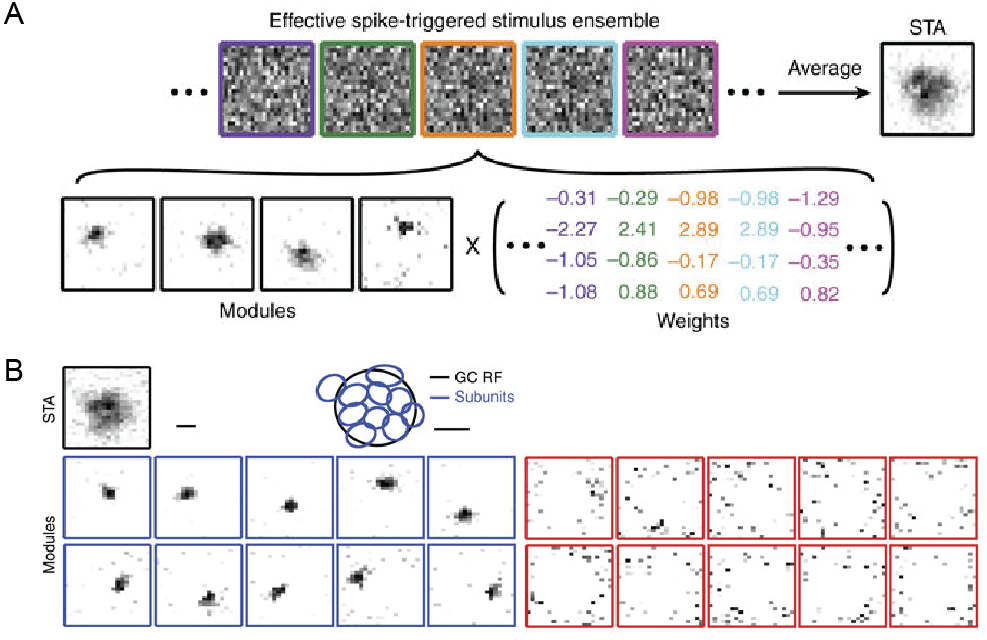
\includegraphics[width=\textwidth]{fig-rev1-retina}
    \caption{
    \revise{Identification of retinal ganglion cell subunits 
    with \ac{STNMF} (adapted from \cite{Liu2017}).
    \textbf{\emph{A}},
	     Samples of a ganglion cell’s effective spike-triggered stimulus ensemble (top),
         whose average corresponds to the cell’s \ac{STA}.
         For easier visual comparison with the subunits,
         \acp{STA} are displayed with negative pixel values set to zero and
         with zero corresponding to white in the grayscale image.
         \ac{STNMF} decomposes this ensemble into a set of modules and 
         a weight matrix (bottom).
         The example here shows four modules that were identified for
         a sample ganglion cell.
    \textbf{\emph{B}},
         Modules obtained for another sample ganglion cell by applying \ac{STNMF}
         with 20 modules (bottom 2 rows). Some modules have a strongly localized structure 
         (blue frames), others are more noise-like (red frames).
         The top row shows the cell’s receptive field,
         given by the spatial component of the STA, as well as the fitted \ac{RF} outline
         (GC RF, black ellipse), together with outlines of the localized subunits 
         (blue ellipses). Scale bars, 100 µm.
    }}
	\label{fig:NMF|retina}
\end{figure}

% Following testing on ground truth data, the researchers recorded spikes from
% \emph{in vitro} retinal ganglion cells
% while the cells were exposed to still photographs and videos of natural scenes.
% \revise{They then applied two classes of factorization methods to the data that can be described as tensor factorization (in which the input is decomposed into separate spatial and temporal features) and matrix factorization (in which the input is decomposed into one unified spatiotemporal module). Most importantly, they applied two kinds of \ac{NMF}, space-by-time (tensor) \ac{NMF} as well as basic (matrix) \ac{NMF} \cite{Onken2016}.}
% \revise{Space-by-time \ac{NMF} works the same way as basic \ac{NMF}, except the input matrix is decomposed into two weight matrices \textbf{$W_{temporal}$} and \textbf{$W_{spatial}$} instead of a single spatiotemporal \textbf{W}, as well as the hidden coefficient matrix \textbf{H}. Space-by-time \ac{NMF} yielded sparser and more compact representations compared to the other techniques, including basic \ac{NMF}.}

\revise{As mentioned in the previous section,
\ac{NSC} has been extensively applied to early visual cortex,
where it has successfully explained 
orientation and frequency tuning of simple and complex cells in \ac{V1} \cite{Hoyer2003},
edge-like pooling of spatial frequency channels in V1 \cite{Hyvarinen2005},
including \ac{RF} properties such as end-stopping and contour integration 
\cite{HoyerHyvarinen2002}.
With the exception of face processing in \ac{IT}
\cite{LeeSeung1999,ChangTsao2017},
\ac{NSC} has yet to be applied to higher-order areas in the ventral visual stream.
The success of \ac{NSC} in explaining V1 and V2 response properties
suggests that it might be possible to extend the model to texture integration in
V4.}


\begin{figure}[!b]
	\centering
	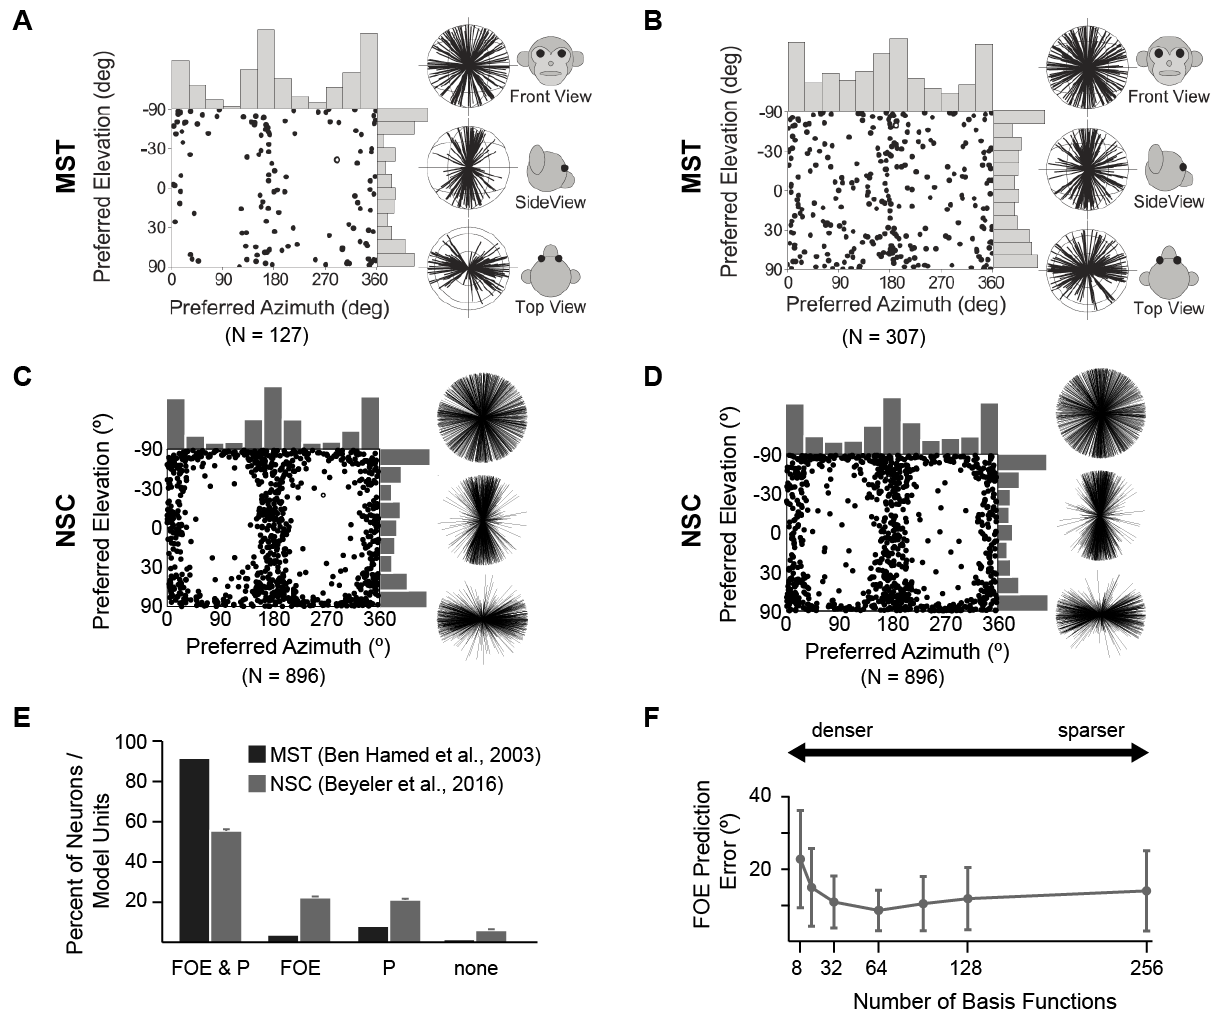
\includegraphics[width=0.97\textwidth]{fig-rev1-MST}
    \caption{
    \revise{
    \textbf{\emph{A-D}},
         Distribution of 3D direction preferences of macaque \ac{MSTd} neurons
         (rotation, \textbf{\emph{A}}; translation, \textbf{\emph{B}}; 
         reprinted from \cite{Takahashi2007})
         and model units in the \ac{NSC}-based sparse decomposition model
         (rotation, \textbf{\emph{C}}; translation, \textbf{\emph{D}}; 
         reprinted from \cite{Beyeler2016}).
         Each data point in the scatter plots corresponds to the preferred azimuth
         (abscissa) and elevation (ordinate) of a single neuron.
         Histograms along the top and right sides of each scatter plot show the
         marginal distributions.
         Also shown are 2D projections (front view, side view, and top view)
         of unit-length 3D preferred direction vectors (each radial line represents
         one neuron).
    \textbf{\emph{E}},
         Distribution of focus of expansion (FOE) and pursuit (P) selectivities
         in macaque \ac{MSTd} (dark gray) and model \ac{MSTd} (light gray;
         reprinted from \cite{Beyeler2016}).
         Neurons or model units were involved in encoding heading (FOE),
         eye velocity (P), both (FOE \& P), or neither (none).
    \textbf{\emph{F}},
         Heading prediction (generalization) error as a function of the
         number of basis functions using 10-fold cross-validation.
         Vertical bars are the SD (reprinted from \cite{Beyeler2016}).
    }}
	\label{fig:NMF|MSTd}
\end{figure}

\revise{In our own work, we found evidence for \ac{NSC} in the dorsal visual stream.
Specifically, we demonstrated that simulated neurons 
in a \ac{NSC} based model of \ac{MSTd} 
responded to  large optic flow fields in much the same way as real neurons in macaque \ac{MSTd} \cite{Beyeler2016}.
Fig.~\ref{fig:NMF|MSTd} shows the distribution of direction preferences
of \ac{MSTd} cells (Fig.~\ref{fig:NMF|MSTd}A, B; \cite{Takahashi2007})
and \ac{MSTd}-like model units (Fig.~\ref{fig:NMF|MSTd}C, D; \cite{Beyeler2016})
for visual translation and rotation.
Each data point in the scatter plots specifies the preferred 3D direction
of a single neuron or model unit.
Histograms along the boundaries show the marginal distributions of azimuth
and elevation preferences.}
Not only did individual units match response properties of individual neurons
in macaque \ac{MSTd},
but the model was able to recover statistical properties of the \ac{MSTd}
population as a whole, such as a relative overrepresentation of lateral
headings (Fig.~\ref{fig:NMF|MSTd}C, D).

\revise{\ac{MSTd} is known to encode a number of perceptual variables,
such as the direction of travel (heading) and eye rotation velocity.
During forward movement, retinal flow radiates out symmetrically from a single point,
the focus of expansion (FOE), from which heading can be inferred.
However, instead of consisting of a set of distinct subpopulations,
each specialized to encode a particular perceptual variable,
\ac{MSTd} has been found to consist of neurons that act more like basis functions,
where a majority of cells were involved in the simultaneous encoding of multiple
perceptual variables (Fig.~\ref{fig:NMF|MSTd}E).
A similar picture emerged when we investigated the involvement of \ac{MSTd}-like
model units in the encoding of both heading and eye rotation velocity
(Fig.~\ref{fig:NMF|MSTd}E).}
% Like most neurons in macaque \ac{MSTd},
% most \ac{MSTd}-like model units were involved in the encoding
% of both heading (FOE) and simulated eye rotation velocity (pursuit, P),
% and only a minority of units contributed to the encoding of only one variable
% or the other.}

\revise{Interestingly, the sparsity regime in which model \ac{MSTd} achieved the
lowest heading prediction error (Fig.~\ref{fig:NMF|MSTd}F) was also the
regime in which \ac{MSTd}-like model units reproduced a variety of known
\ac{MSTd} visual response properties
(for experimental details refer to \cite{Beyeler2016}).
In contrast to findings about early visual cortex,
this regime does not use an overcomplete basis set \cite{OlshausenField1996},
yet can still be considered a sparse coding regime \cite{SpanneJorntell2015}.
Such an intermediary sparse code might be better suited
(as opposed to an overcomplete basis set)
for areas such as \ac{MSTd},
because the increased memory capacity of such a code might lead to compact
and multifaceted encodings of various perceptual variables
\cite{BenHamed2003}.}




\subsection*{\revise{NSC in the Auditory cortex}}

\revise{The auditory cortex is a prime example of efficient coding. The auditory system is believed to decompose auditory signals into
a set of elementary acoustic features \cite{SmithLewicki2006},
such that the complete acoustic waveform can be described by a
sparse population code that operates near an information-theoretic optimum
\cite{SmithLewicki2006,rokem2006,Hromadka2008}.
It is therefore not surprising that computational models based on \ac{NSC}
have been very successful at describing the spectro-temporal \acp{RF}
of neurons in the \ac{A1} \cite{Martinez2015,David2007}.
Response properties of \ac{A1} neurons are well described by a spectrogram;
they are often tuned to stimulus frequency but are rarely phase-locked
to oscillations of the sound waveform \cite{Leaver2010}.
The cortical representation of auditory signals seems to not only be sparse,
but also rely on statistically independent acoustic features \cite{Klein2003}.}

\revise{Similar to visual cortex, auditory cortex is hierarchically organized,
with neurons in \ac{A1} responding to simple acoustic features of natural sounds,
and higher-order areas responding to more behaviorally relevant stimuli.
The anterior superior temporal region of auditory cortex, for example,
responds to categories of acoustic objects,
such as sounds produced by voices and musical instruments
\cite{Leaver2010}.
An intriguing question for future modeling studies is therefore 
whether \ac{NSC} can be extended to the next level of the auditory hierarchy:
Would it be possible to construct more complex acoustic objects from a sparse,
parts-based set of elementary, \ac{A1}-like acoustic features?
And would the representation of such acoustic objects resemble neuronal responses
in the anterior superior temporal region of auditory cortex?}

% \revise{The primary auditory cortex
% % similar to the early visual cortex and somatosensory cortex,
% % \mikeNote{A1 is actually higher up in the auditory hierarchy than V1 is in the visual hierarchy. I think the same is true for S1. Confusing to compare them}
% may also feature parts-based representations, hinted at by the tonotopic organization of the region, which been determined through multiple neuroimaging studies in humans, as well as in electrophysiological recordings in nonhuman primates \cite{humphries2010,bendor2008}. This functional organization is reminiscent of the organization of early visual cortex. Likewise, studies of auditory cortex support a hierarchically organized pathway, with more complex acoustic objects represented higher up the hierarchy. In support of this idea, the anterior superior temporal region of auditory cortex exhibits sensitivity to categories of acoustic objects (such as sounds produced by voices or by musical instruments), while neurons in regions that are closer to the primary auditory cortex operate more like feature detectors, responding to acoustic features of natural sounds 
% \cite{Leaver2010}. Additionally, sparse coding for vocalizations has been found in the primary auditory cortex of marmoset monkeys, supporting the usage of sparse coding principles for behaviorally relevant sounds \cite{Terashima2013}.}


% \revise{The auditory cortex seems to rely on precise spike timing for efficient information transmission based on experiments that have examined the stimulus-response joint probability distribution in grasshoppers. Findings suggest that the information transmission rate of auditory receptor neurons increase with the amplitude modulation of a stimulus. Furthermore, naturalistic stimuli were encoded suboptimally as compared to idealized Gaussian stimuli, suggesting that auditory receptor neurons encode specific behaviorally relevant stimulus features, consistent with a system that is minimizing metabolic energy costs \cite{rokem2006}. Another finding from awake, behaving rats confirms the sparse population representation of sounds and found that fewer than 5\% of neurons were active at any given time, with most stimuli eliciting high firing rates, but some eliciting very low firing rates in some neurons \cite{Hromadka2008}.}

% \begin{figure}[!h]
% 	\centering
% 	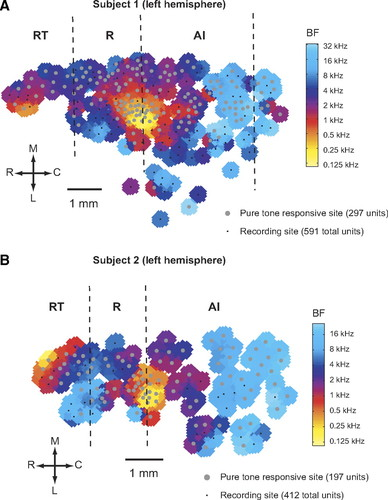
\includegraphics[width=\textwidth]{auditoryTonotopic}
%     \caption{\revise{Reproduced from Bendor et al. 2008 \cite{bendor2008}. Tonotopic organization of neuronal responses to tones of varying frequency in two marmomset monkeys. AI = primary auditory cortex, R = rostral field, and RT = rostrotemporal field. These primary fields are referred to as the `core regions' of auditory cortex. They are heavily interconnected and receive input from one another and from the thalamus, which supports tonotopic organization. The presentation of low to high frequency tones of varying purity results in a gradient of frequency sensitivity across the three fields.}}
% 	\label{fig:auditoryTonotopic}
% \end{figure}

% \revise{The primary auditory cortex
% % similar to the early visual cortex and somatosensory cortex,
% % \mikeNote{A1 is actually higher up in the auditory hierarchy than V1 is in the visual hierarchy. I think the same is true for S1. Confusing to compare them}
% may also feature parts-based representations, hinted at by the tonotopic organization of the region, which been determined through multiple neuroimaging studies in humans, as well as in electrophysiological recordings in nonhuman primates \cite{humphries2010,bendor2008}. This functional organization is reminiscent of the organization of early visual cortex. Likewise, studies of auditory cortex support a hierarchically organized pathway, with more complex acoustic objects represented higher up the hierarchy. In support of this idea, the anterior superior temporal region of auditory cortex exhibits sensitivity to categories of acoustic objects (such as sounds produced by voices or by musical instruments), while neurons in regions that are closer to the primary auditory cortex operate more like feature detectors, responding to acoustic features of natural sounds 
% \cite{Leaver2010}. Additionally, sparse coding for vocalizations has been found in the primary auditory cortex of marmoset monkeys, supporting the usage of sparse coding principles for behaviorally relevant sounds \cite{Terashima2013}.}



\subsection*{\revise{NSC in the Olfactory cortex}}

\revise{In contrast to most other sensory modalities, 
the basic perceptual dimensions of olfaction remain unclear.
Odors evoke complex responses in granule cells (located in the olfactory bulb)
that evolve over hundreds of milliseconds \cite{Broome2006}.
Granule cells use a sparse combinatorial code to convey information about odor identity
and concentration \cite{Koulakov2011,Gupta2015}.
% \revise{ The segregated odor mapping contained in the olfactory bulb is then transmitted to the piriform cortex (considered specialized for olfaction), which is thought to be where odor object percepts are formed \cite{chen2014,stettler2009}. The piriform cortex does not exhibit a topographic organization scheme (thus there is no clustered or graded pattern of response that can be mapped), but neurons in this region nonetheless elicit unique but overlapping ensemble-based responses to odorants \cite{stettler2009}. However, a spatial structure can be discerned when examining the projections of output neurons in the piriform cortex, which are highly segregated and functionally specific \cite{chen2014}.}
Downstream from the olfactory bulb, odors tend to activate a small but consistent
proportion ($\sim 10\%$) of cortical neurons in the piriform cortex \cite{poo2009},
which is thought to form odor object percepts \cite{chen2014,stettler2009}.
% \revise{In rat piriform cortex, odors evoke sparse ensemble activity across the population that results from an imbalance between excitation and inhibition (excitation is uncommon and odor-specific, while inhibitory responses are widespread and broadly tuned) \cite{poo2009}, a finding that is also observed in awake, behaving mice \cite{rinberg2006}. Odors tend to activate a small but consistent proportion of cortical neurons in the piriform cortex (9 to 11\%). Furthermore, olfactory cortical neurons responded selectively to stimuli, and population responses to odors were very sparse, providing evidence for both lifetime and population sparseness in the olfactory cortex \cite{poo2009}.}
% \mikeNote{we don't want to anger reviewer  with population sparseness}
Although piriform cortex is not topographically organized,
a spatial structure can be discerned when examining the projections of output neurons,
which are highly segregated and functionally specific.
Whereas the anterior piriform cortex is associated with the encoding of 
odor identity and odor structure, 
the posterior piriform cortex is involved in associational aspects of odors, 
such as valence and similarity \cite{chen2014,gottfried2006}.}
% \revise{It has also been observed that the anterior and posterior piriform cortex are differentially involved in odor processing. The anterior piriform cortex is associated with the encoding of odor identity and odor structure, while the posterior piriform cortex is involved in associational aspects of odor, such as valence and similarity \cite{chen2014,gottfried2006}. The olfactory bulb and piriform cortex also seem to have highly context-dependent and multimodal odor representations \cite{fournel2016,mandairon2014}, consistent with the hypothesized role of the piriform cortex as an association cortex for odor objects.}
% \revise{Finally, there exists computational evidence to support nonnegative sparse coding in the olfactory cortex. In a simple spiking neural network model designed to measure causal inference, researchers found that this spiking network could solve high-dimensional quadratic optimization problems with nonnegativity constraints for feature detection via an 'explaining away' mechanism. They use odor detection as a concrete example of a problem that this network might solve, and suggest that this kind of coding may be employed by olfactory bulb granule cells \cite{MorenoBoteDrugowitsch2015}.}

\begin{figure}[!b]
	\centering
	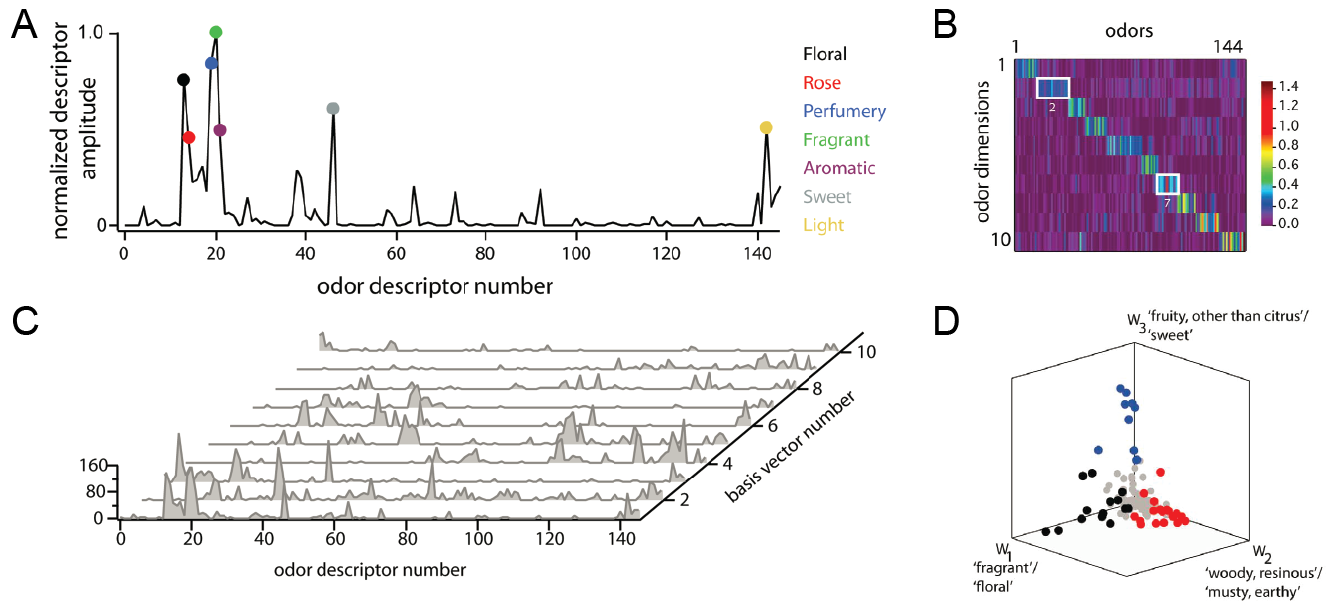
\includegraphics[width=\textwidth]{fig-rev1-olfaction}
    \caption{\revise{\ac{NMF} recovers a sparse and parts-based representation
    of olfactory perceptual space (reprinted from \cite{Castro2013}).
       \textbf{\emph{A}},
          Plot of normalized odor descriptor amplitude vs. odor descriptor number for
          the first basis function. Each point along the x-axis corresponds to a single
          odor descriptor, and the amplitude of each descriptor indicates the
          descriptor's relevance to the shown perceptual basis function.
          Colored circles show the 7 largest elements, with corresponding descriptors
          listed on the right.
       \textbf{\emph{B}},
          Waterfall plot of the 10 basis functions constituting \textbf{W}.
       \textbf{\emph{C}},
          Heat map of the coefficient matrix, \textbf{H},
          where each column of \textbf{H} corresponds to a different odor.
          Columns of \textbf{H} are normalized and sorted into groups defined by
          peak coordinate (1-10).
       \textbf{\emph{D}},
          Plot of all 144 odors in the dataset (each point is a column in \textbf{H})
          in the space spanned by the first three basis functions.
          Black, red, and blue points are those with peak coordinates in dimensions
          1, 2, and 3, respectively. Gray points are all remaining odors.}}
	\label{fig:evidence-olfaction}
\end{figure}

\revise{Castro and colleagues \cite{Castro2013} provided 
one of the most compelling pieces of evidence for \ac{NSC}
in the olfactory system to date:
In an effort to elucidate the dimensions along which perceptual space might be
organized in the olfactory system,
they applied \ac{NMF} to a dataset of 144 monomolecular odors,
each represented by a 146-dimensional odor profile.
Each dimension in the odor profile corresponded to the rated applicability of
a number of semantic labels, such as `sweet', `floral', and `heavy'
(Fig.~\ref{fig:evidence-olfaction}A).
By applying \ac{NMF} to the odor profile, they showed that a small, sparsely active set of basis functions could accurately describe any odor in the dataset
(Fig.~\ref{fig:evidence-olfaction}C).
Interestingly, \ac{NMF} revealed a prominent block
diagonal structure to the full matrix \textbf{H}
(Fig.~\ref{fig:evidence-olfaction}B), indicating that:
1) a given odor tended to be characterized by a single prominent dimension,
implying that the basis functions recovered by \ac{NMF} were perceptually meaningful,
and 2) all 10 dimensions were occupied,
implying that the basis functions recovered by \ac{NMF} could span the space of
behaviorally relevant odors.
This suggests that a given odor percept may be considered an 
instance of one of several fundamental qualities.
For the data set investigated, individual odor profiles were well-classified 
by their proximity to a single one of these dimensions, 
with all ten dimensions being approximately equally expressed 
across the set of odors.}

\revise{Furthermore, \ac{NMF} recovered basis functions whose descriptors align
with perceptual dimensions highlighted in several previous analyses of odor space,
including but not limited to relative pleasantness (e.g., `fragrant`, `sickening`), 
and potential palatability (`woody, resinous', `chemical', `sweet', and `lemon').
Odors clustered predominantly along these axes
(Fig.~\ref{fig:evidence-olfaction}D), 
motivating the interpretation that odor space is organized 
by a relatively large number of independent qualities that apply categorically
\cite{Castro2013}.}


\subsection*{\revise{NSC in the Somatosensory cortex}}
%* Somatosensory cortex - Evidence from barrel cortex in rats (Spatial organization of neuronal population responses in layer 2/3 of rat barrel cortex) and from somatosensory in cats and bats
\revise{Evidence for a \ac{NSC} mechanism in somatosensory cortex exists for multiple species. First, the presence of a topographically organized sensory 'homunculus' in human and bat somatosensory cortex (as well as rat somatosensory, or barrel, cortex) \cite{penfield1937,hari1993,chadha2011,petersen2007} suggests a possible parts-based representation scheme. Second, sparse and efficient coding schemes have been observed in mouse barrel cortex (in one study, 10\% of recorded neurons were active for 50\% of all recorded spikes) \cite{oconnor2010}, with heightened sparsity in an associative fear learning task \cite{gdalyahu2012}. Finally, something akin to mixed selectivity may also be utilized in human somatosensory cortex, according to a non-invasive neuromagnetic imaging study of a high-precision motor task (handwriting). The data suggested rapid modulation of task-specific involvement of somatosensory neurons might be due to the dynamic online selection of pre-existing somatosensory maps \cite{braun2001}. This is further supported by the presence of converging multimodal inputs from disparate regions to somatosensory cortex as observed in cats\cite{kang1985}.}
% \emilyNote{Wondering if (and how) we should address the fact that these early sensory areas are greatly expanded compared to the areas of input)}




\subsection*{\revise{Parietal cortex}}

\revise{Analogous to our modeling work in \ac{MSTd} \cite{Beyeler2016},
it might be possible to apply \ac{NSC} to other areas of the posterior parietal
cortex that are involved in multisensory heading perception.
Areas such as the \ac{VIP} and \ac{VPS} are also known to respond to optic flow,
but they increasingly respond to inertial vestibular stimulation as well
\cite{Chen2011}.
Although the sparseness of the population code in \ac{VIP} and \ac{VPS} is not known,
the fact that neurons in these areas respond to mixtures of visual and vestibular
heading cues make them prime examples 
to be examined with an \ac{NSC} based modeling approach.}

\revise{Elsewhere in parietal cortex, single neurons act as basis functions 
to represent the spatial configuration of objects 
with respect to multiple reference frames
(e.g., by transforming eye-centered to body-centered coordinates).
\cite{Poggio1990,PougetSejnowski1997,PougetSnyder2000}.
This is similar to the integration of multimodal heading cues mentioned above,
as well as to other associative areas such as \ac{RSC},
which demonstrates conjunctive coding of various spatial navigation cues
\cite{AlexanderNitz2015,Rounds2018}.
There is further evidence that actions are represented in parietal cortex
with respect to arbitrary and abstract reference frames, 
such as with respect to a planned route through an environment \cite{nitz2009parietal}.
From a theoretical standpoint, \ac{NSC} seems a good candidate to find an efficient,
reference-frame agnostic representation of various behaviorally relevant variables
\cite{LouieGlimcher2012,louie2015adaptive,andersen1997multimodal,BenHamed2003},
but future studies will have to address these issues step by step.}


% This allows the transformation of representations from eye-centered to body centered coordinates, and provides a mapping from sensory inputs to motor actions . Such function is similar to the representation of multiple spatial frames of reference in retrosplenial cortex, and like the retrosplenial cortex, the parietal cortex has long been thought of as an association area for the representation of space based on multimodal sensory inputs. There is further evidence that actions are represented with respect to arbitrary and abstract reference frames, such as with respect to a planned route through an environment \cite{nitz2009parietal}. The construction of arbitrary reference frames appears to be possible due to the flexible combination of sensory inputs including head direction, eye position, vestibular information, auditory cues, and other information \cite{andersen1997multimodal}, which is again reminiscent of findings in retrosplenial cortex \emilyNote{well, other way around, really...}. There also appears to be value-related coding in the parietal cortex to support decision-making \cite{louie2015adaptive}.}
% \emilyNote{no apparent evidence for sparse coding in parietal that I could find.}

% * The whole business on basis functions (Pouget, Snyder)
% * Louie and Glimcher
% * These could be relevant:
% \cite{Poggio1990,PougetSejnowski1997,PougetSnyder2000}



% \subsection*{\revise{Gustatory cortex}}
% \mikeNote{After a long back and forth, I am against this section. OK it looks intriguing because of similarity to olfactory and parietal cortex, but it's a blue ocean. We don't know anything. There are no models. Why waste space on it?}
% \revise{Despite its similarities to information processing 
% in the olfactory system and parietal cortex,
% gustatory cortex has received relatively little attention
% from an \ac{NSC} viewpoint.
% Gustatory cortex is a multimodal brain region that integrates olfactory
% as well as somatosensory information \cite{DeAraujo2009}
% to give rise to several classes of taste quality
% (e.g., sweet, salty, bitter, sour, umami) \cite{lemon2007}.
% Reminiscent of odor processing in the olfactory bulb,
% taste receptor cells are selective for different classes of chemicals,
% with gustatory fibers maintaining a high degree of specificity
% when carrying taste information into the brain \cite{smith2008central}.
% This functional segregation suggests the existence 
% of a parts-based representation of taste quality.
% Furthermore, taste representations in the gustatory system rely on 
% precise spike time coding \cite{lemon2007},
% suggesting that taste is encoded using a sparse code.
% However, more research is needed to elucidate the underlying coding principles.
% }

% \revise{In gustatory cortex, the picture is similar. 
% It is a target for multimodal input and seems to be a site for multimodal sensory integration. Temperature, valence, texture, and other features are all encoded in the gustatory cortex, including olfactory and somatosensory information \cite{DeAraujo2009} to give rise to several classes of taste quality (e.g., sweet, salty, bitter, sour, umami) \cite{lemon2007}. It is believed to be the case that taste receptor cells are selective for different classes of chemicals, and that taste receptors are distributed in a segregated manner, reminiscent of the olfactory bulb, and that a high degree of specificity is maintained in the gustatory fibers that carry taste information into the brain \cite{smith2008central}. Furthermore, taste representations in the gustatory system seem to rely on precise spiking and temporal information \cite{lemon2007}. These findings support a sparse lifetime coding scheme in the gustatory system, though there has been argument over this view \cite{smith2008central}. In the gustatory cortex, this gives rise to ensemble representations that contain both narrowly and broadly tuned neurons \cite{carleton2010}. Consequently, sparse ensemble activity seems likely in this region, but no clear or definitive evidence exists to our knowledge.} \emilyNote{trying to avoid the 'sparse = specific, segregated, highly selective' and 'sparse = small subset of neurons active' confusion, not sure I've succeeded} \revise{Neuroimaging and electrophysiological recording studies in human and non-human primates have shown that highly overlapping ensembles of neurons seem to encode taste quality, but that there are also much more clearly spatially organized representations of pleasantness and unpleasantness, which can be altered through conditioning \cite{carleton2010}.}% (Fig. ~\ref{fig:GustatoryReps}).}

% \mikeNote{I'm on the fence about this figure and have removed it for now. It doesn't really show NSC in the way that e.g. the olfactory figure does.}

% \begin{figure}[h]
% 	\centering
% 	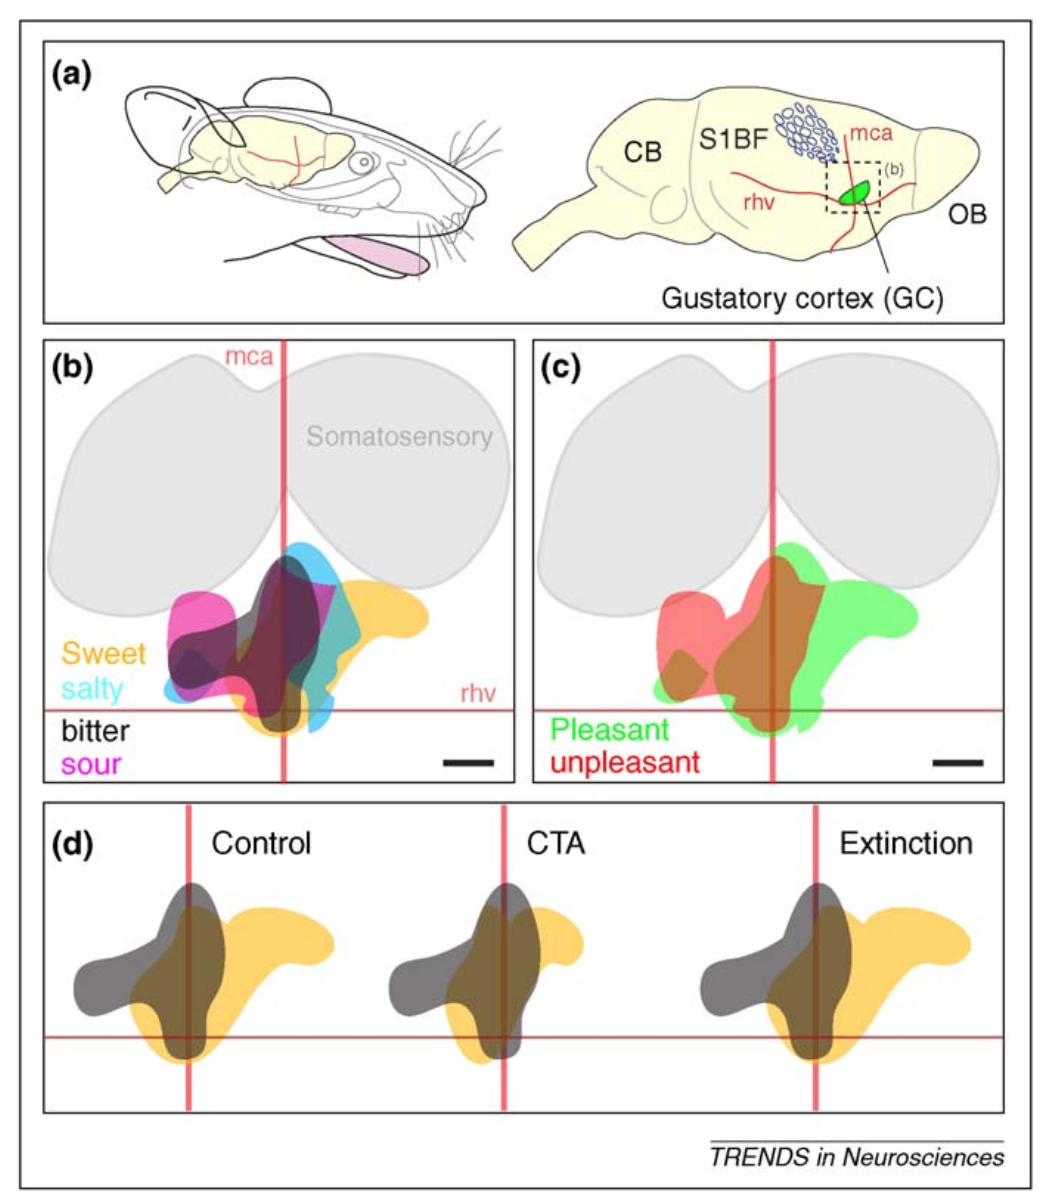
\includegraphics[width=0.8\textwidth]{gustatoryRepresentations}
%     \caption{\revise{Reproduced from Carleton et al. \cite{carleton2010}.
%        \textbf{\emph{A}},
%           Cartoon drawing of the location of the gustatory cortex 
%           in the rat brain. 
%        \textbf{\emph{B}},
%           Representations of flavors categorized as sweet, sour, bitter, 
%           or salty have topographical but overlapping representations, 
%           suggesting that the region contains ensemble representations 
%           with both broadly and more narrowly tuned neurons.
%        \textbf{\emph{C}},
%           Hedonic value is also encoded in gustatory cortex, with unpleasant
%           and pleasant tastants having much more distinctly organized 
%           representations that change with aversive conditioning, 
%           as determined by imaging studies. }}
% 	\label{fig:GustatoryReps}
% \end{figure}




\subsection*{\revise{Parts-Based Dimensionality Reduction in the Retrosplenial cortex (RSC)}}

\revise{There is increasing evidence that \ac{NSC} can also explain 
response properties in \ac{RSC}, an area important for navigation and spatial memory \cite{Miller2014,Nelson2015,VannAggleton2009}.
As mentioned above, neurons in the \ac{RSC} conjunctively encode multiple variables related to the environment and one's position and movement within it, allowing for the representation of environmental features with respect to multiple spatial reference frames \cite{AlexanderNitz2015}. The \ac{RSC} may also conjunctively encode information about reward in combination with navigation and spatial information \cite{vedder2016}.}

\revise{In the present paper, 
we applied NMF to the behavioral data from the original
\ac{RSC} experiment conducted by Alexander and Nitz \cite{AlexanderNitz2015}
(for experimental details, see Supplementary Materials).
\mikeNote{After the latest edits,
I am still confused as to what is in Rounds 2018.
If any of this is now published, we should refer to the published material
instead. Having a Supplementary Materials section with original research
(in a review article) is a bit awkward...}
\jeffNote{This section is confusing.  There were no neurons in the the NMF application to RSC. I re-wrote the first paragraph, but I am not sure where those numbers are coming from in the second paragraph. }
Using this method, we were able to reduce the dimensionality of the input space from 417 behavioral inputs to 30 basis vectors, and found a close correspondence to the functional patterns of activation between the basis units and the patterns observed in the dataset. Additionally, activity computed from the basis units could be used to replicate the population behavior of the dataset \cite{AlexanderNitz2015}. We found that model neuron activity could replicate the population behavior of the dataset.}

\revise{We also considered the sparsity of activity in both the experimental data and our model. In the experimental dataset, we found that only 16.3\% of neurons were active for each combination of inputs, while in the \ac{NMF} model, approximately 10\% of the model units (ranging from 3 to 4 out of 30) were active per stimulus combination. Sparse representations of spatial context in the retrosplenial cortex have also been reported elsewhere \cite{mao2017}.} 


% \mikeNote{I don't think we should consider place cells `parts-based', it's more like a labeled line/local code (you're either in a certain location or not). Check Fig. 1B: Do individual place cells encode parts of places? Can you infer where you are in the environment by being 10\% in the location encoded by neuron A plus 20\% in the location encoded by neuron B? I don't think so. Grid cells on the other hand... ;-)}

% \emilyNote{I'm not sure I understand the distinction between labeled line and parts-based, then. Isn't 'parts-based' just shorthand for segregated/partitioned representation of an input space? Also that seems like it may destroy our case for auditory/olfactory/gustatory cortex, where all the papers I read frequently described the nature of inputs as labeled line. Also, no grid cells in RSC, only in entorhinal, so I'm not sure how to make the argument for parts-based representations in RSC besides saying 'well our model says it could be.'}

% \emilyNote{I looked at statistics in the experimental RSC data, found that if you look at the average FR per neuron across trials, 29\% of cells are active. If you look for neurons that fire > 3Hz at least once over the course of a trial, it's more like 50\% active. If you look at response on a bin-by-bin basis, it's 16\%.
% However, as part of preprocessing, Alexander and Nitz threw out all completely silent neurons in the dataset.}



\subsection*{\revise{Prefrontal cortex (PFC)}}
\jeffNote{The first 2 paragraphs say nothing about NMF or NSC.  Is the evidence strong in the PFC?  I would consider deleting this section.}
\revise{\Ac{PFC} is thought to play a fundamental role in 
flexible, context-dependent behavior,
but the exact nature of the computations underlying this role 
remains large unknown \cite{Mante2013}.
Individual \ac{PFC} neurons typically encode multiple task-related signals
at once, including the animal's upcoming choice, the context,
and the strength of the sensory evidence \cite{Mante2013,Rigotti2013,Kobak2016},
defying a deep understanding of how 
individual \ac{PFC} neurons contribute to behavior.
Researchers have argued that high-dimensional neural representations
enable simple readout mechanisms such as linear classifiers to implement
a large set of input-output relations \cite{Rigotti2013,Barak2013}.}

\revise{The most successful modeling studies in \ac{PFC} have asked
whether the confounding single-neuron responses could be understood as
views of a simple dynamical process at the population level
\cite{Mante2013}.
They found that \ac{PFC} population responses dynamically encode several task variables underlying an animal's behavior.
During decision making, the response to a choice stimulus is characterized
by an initial stimulus-specific population response,
but evolves to different final decision related
states depending on the current rule \cite{Stokes2013}.}

\revise{While there is evidence of dimensionality reduction 
in \ac{PFC} \cite{Mante2013},
little is known about the sparsity of the population code.
The only evidence for sparse coding is restricted to the \ac{mPFC} in rats
\cite{Fujisawa2008,Wei2015},
an area that is engaged in working memory tasks 
and sensitive to the expectation of reward \cite{Baeg2003}.
Whereas \ac{NMF} was able to elucidate functional properties of the \ac{mPFC}
network while rats behaved in a Y-maze \cite{Wei2015},
the study also highlighted the dependence of \ac{mPFC} network activity
on the animal's choice behavior.}



% \revise{Neurons in the \ac{mPFC} are engaged in working memory tasks 
% and have been shown to be sensitive to the expectation of reward \cite{Baeg2003}. 
% Motivated by the observation that functional changes in a network must be observed to understand neural processing and the importance (or unimportance) of particular anatomical connections, Wei and colleagues \cite{Wei2015} used \ac{NMF} to find an efficient description of
% \ac{mPFC} network properties. Their findings highlight that the mPFC network is sparse and that population activity could be described by basis functions corresponding to a low-dimensional portion of the original space.
% Their result suggests that \ac{NMF} faithfully captured the patterns of mPFC network activity, enabling them to study network dynamics in a way that would not have been possible in the original high-dimensional space.}



\subsection*{\revise{Motor cortex}}
\jeffNote{Same comment as in PFC.  Just because its sparse or parts-based does not imply NMF or NSC.  This doesn't seem like a strong argument.}
\revise{As in the somatosensory cortex, there exists a topographic partitioning of 
\mikeNote{I suspect this section is not strong enought for Reviewer 1, who seems to know an awful lot about motor cortex}
representations of the body in the primary motor cortex, referred to as the motor homunculus \cite{penfield1937,metman1993}. This constitutes evidence for the existence of parts-based representations in at least some parts of motor cortex, in combination with studies that show the activity patterns associated with small sets of neurons in primary motor cortex represent naturalistic movements, and can be used to reconstruct joint angles \cite{Vargas2010decoding}. The organization of the motor cortex as it progresses past primary motor is less clear, but some researchers suggest that these regions can be well-described using nearest-neighbor similarity \cite{GrazianoAflalo2007}. They argue that topographical organization is easy to accomplish when the input space to be mapped is two-dimensional like the cortical sheet, but as input spaces become increasingly high-dimensional, topograhic organization disappears as different inputs and combinations of inputs compete for representation. Using a model that was initially organized somatotopically, the researchers studied the self-guided reorganization of the map in response to hand position and a set of movement dimensions that corresponded to those movements a monkey would be physically able to perform. They found that principles of nearest-neighbor similarity described the way that such a high-dimensional space was mapped onto a two-dimensional surface, and which reflected the actual organization of the motor cortex, and was constituted of sets of parts-based representations \cite{GrazianoAflalo2007}.} 

\revise{This idea also appears to be consistent with the somatosensory and motor representations of arms and movement in octopuses, who do not have topographically organized sensorimotor maps. Instead, their nervous system structure is centralized, with body part and movement representations being highly distributed \cite{zullo2011}. There is a hierarchical organization evident, with highly stereotyped movement circuits at the periphery and distributed but overlapping parallel pathways at the center for higher motor control, which likely integrate sensory inputs. Thus the octopus can efficiently execute commands via the central control pathways that then execute automated movements in the individual arms. This structure and organization appears consistent with the nearest-neighbor similarity concept of organization described by Graziano and Aflalo \cite{GrazianoAflalo2007}.}
% We suggest that it would be interesting and compelling to see if such self-organizing models might describe the sensorimotor systems of octopuses and other 'dynamically embodied' \cite{zullo2011} species.} 

\revise{Evidence for sparse coding in the motor cortex, on the other hand, is lacking---in fact, some studies suggest that most neurons are active in motor cortex during movement preparation and support a basis set by which many movement parameters are represented \cite{churchland2007}.
The role of neurons that do not explicitly represent any movement parameters
can be explained by recent work based on optimal feedback control theory, 
which postulates that the goal of motor cortex is to produce a desired movement and force, taking into account the state of the muscles \cite{Gallego2017}.
This hypothesis avoids the need for explicit representation 
of movement parameters covariates by single neurons,
although some neurons may still represent some movement parameters
as a byproduct of the necessary control signals
\cite{Gallego2017}.}

% However, while the lack of sparse activation is a limitation for 
% ac{NSC}, it has also been observed that sets of neuronal activations across the population cancel each other out, a proposed mechanism by which movements are planned in motor cortex without execution \cite{Kaufman2014}. This is a functionality that could possibly be described really well by \ac{NSC}, because the weighted sum of the underlying parts-based representations and activity patterns could naturally give rise to this phenomenon.
% \mikeNote{Huh? This makes no sense. NSC can't do subtractions.}





\subsection*{\revise{Hippocampus}}

\jeffNote{Same comment as in PFC and motor cortex.  Just because its sparse or parts-based does not imply NMF or NSC.  This doesn't seem like a strong argument. You may want to have a section called "Other areas" that states there is evidence for dimenionality reduction, parts-based representations, and sparse activity in the PFC, motor cortex, and hippocampus. Future studies may show that features can be recovered by applying NSC to the inputs of these regions.}
\revise{The CA1 region of the hippocampus have long been thought of as an auto-associative network that automatically performs pattern completion in response to partial inputs \cite{rolls2013}, while the dentate gyrus and hippocampal CA3 are believed to perform pattern separation in order to sparsify and decorrelate the entorhinal inputs coming into the hippocampus \cite{Bakker2008}. This orthogonalization of overlapping input patterns is thought to underlie the formation of episodic memories and the discrimination of similar environmental contexts by the hippocampus \cite{myers2011pattern}. Likewise, activity in both the dentate gyrus granule cells and in pyramidal cells in hippocampal CA1/CA3 subfields is sparse \cite{Poli2017}.
In support of a parts-based representation scheme, hippocampal neurons exhibit conjunctive encoding and mixed selectivity properties similar to those observed in retrosplenial cortex \cite{komorowski2009,mckenzie2014}.}



\subsection*{\revise{NSC in the Basal ganglia}}

\revise{The basal ganglia are a cluster of nuclei containing the striatum, globus pallidus, substantia nigra, and the subthalamic nuclei. They play a prominent role in the coordination of movement, and are implicated in movement disorders such as Parkinson's disease \cite{BarGad2003_Review}. Together, the basal ganglia, the thalamus, and the cortex form a sophisticated loop consisting of multiple convergent and sparsely connected feedforward pathways that preserve segregated topography between the various layers and their inputs \cite{BarGad2003_Review}.}

\revise{Motivated by the observation of high convergence ratios between regions, Bar-Gad et al. \cite{BarGad2000,BarGad2003_Review} developed the Reinforcement-Driven Dimensionality Reduction (RDDR) model to explain these highly convergent pathways in terms of performing dimensionality reduction. They successfully used Hebbian learning to reproduce basal ganglia response patterns associated with reward \cite{BarGad2000}, a function associated with cortico-striato-pallidal circuitry. The authors later applied nonnegativity constraints to the Hebbian learning in the model so that it effectively performed \ac{NMF} on its inputs. The model advanced understanding of the cortico-striato-pallidal loop by capturing behavior of the circuit while explaining the existence of convergent and lateral connections in the region that other models have historically ignored \cite{BarGad2003_Review}.}

\jeffNote{I deleted the sentences about inhibition and learning. Although interesting, it was not pertinent to our NSC perspective.}
\revise{While it has not been clearly reported whether or not activation patterns throughout the basal ganglia are sparse, the maximal connection probabilities between striatal, pallidal, and thalamic neurons are very low ($<$1\%) \cite{BarGad2003_Review}, which may suggest that neurons are also likely to be sparsely activated, and the activity of spiny neurons in the striatum is reportedly sparse \cite{schwab2015}. Corticostriatal neurons in primary motor cortex also exhibit sparse activity \cite{Turner2000}. Parts-based representations seem to exist in the basal ganglia based on the observation of topographical preservation of the kinds of information trasmitted in the basal ganglia. The authors note this with respect to their model, saying that nonnegative matrix factorization provides an encoding more consistent with the topographic innervation and sparse encoding of the basal ganglia \cite{BarGad2003_Review}.}

% \emilyNote{In our table, we had 'X' for sparse, but the referenced papers say basal ganglia has sparse connectivity, not necessarily sparse neural activation. However, Bar-Gad et al say that nonnegative matrix factorization fits better with the 'topographic innervation' and 'sparseness of encoding.'}
% \emilyNote{Might want some other papers in here that aren't Bar-Gad, I guess? Might also need some rewording in some places.}




%as determined by an experiment in which rats ran back and forth on a W-shaped track that occupied two different spatial locations within the room in each recording session to test sensitivity to the allocentric reference frame (i.e., track positions $\alpha$ and $\beta$). Outbound and inbound runs were made up of opposite turn sequences (left-right-left (LRL) and right-left-right (RLR), respectively) that corresponded to different sets of trials, which allowed assessment of sensitivity to the egocentric and route-based reference frames. 

%During the experiment, activity from 228 \ac{RSC} neurons was recorded along with four behavioral metrics: linear velocity, angular velocity, head direction, and allocentric position. Using Gaussian and cosine tuning curves, we created idealized input neurons that encoded these four variables. 

%    In the case of the \ac{RSC}, the basis vectors that resulted from the NMF model produced activation patterns that could be used to infer behavior, suggesting that the model functions in a manner similar to the biological RSC. Because this region responds to multiple spatial frames of reference (egocentric, route-centric, and allocentric) simultaneously, it is possible to accurately reconstruct the position of an animal within a route situated in a specific part of the environment if neural activity for that route is compared with itself. In contrast, if neural activity associated with the same route but situated in different parts of the room are compared, then the reconstruction of position should be poor (for more details, see \citep{AlexanderNitz2015}), showing that the \ac{RSC} distinguishes routes that have different allocentric positions in space. We found that the activity patterns computed using the NMF basis vectors yielded qualitatively similar results when subjected to the same analysis.

% The results were also consistent for the \ac{RSC}. In the neurophysiological dataset, experimentally observed neurons were classified into three broad categories: 
% % these 3 are so incredibly, excruciatingly wordy 
% 1) those that were insensitive to turn-based actions performed by the rats running along the track but nonetheless exhibited complex and robust firing patterns, 2) those that were sensitive purely to turning behaviors performed by the rats such that they responded exclusively to left or right turns, and 3) neurons that demonstrated turn type selectivity, but with increased firing associated with specific instances of the preferred turn type based on their position in the turn sequence associated with the route regardless of the route's location in allocentric space. When \ac{NMF} was applied to the behavioral variables encoded by idealized input neurons, the resulting basis vectors could be categorized into the same functional categories and followed the same approximate distributions as in the experimental dataset (Fig.  \ref{fig:NMF|neuronalresponse}B).


% In the case of the \ac{RSC}, the basis vectors that resulted from the NMF model produced activation patterns that could be used to infer behavior, suggesting that the model functions in a manner similar to the biological RSC. Because this region responds to multiple spatial frames of reference (egocentric, route-centric, and allocentric) simultaneously, it is possible to accurately reconstruct the position of an animal within a route situated in a specific part of the environment if neural activity for that route is compared with itself. In contrast, if neural activity associated with the same route but situated in different parts of the room are compared, then the reconstruction of position should be poor (for more details, see \citep{AlexanderNitz2015}), showing that the \ac{RSC} distinguishes routes that have different allocentric positions in space. We found that the activity patterns computed using the NMF basis vectors yielded qualitatively similar results when subjected to the same analysis.

% The sparsity and nonnegativity constraints of the \ac{NSC} seem to extract similarities between neuronal firing patterns that result in
% consistent and stable representations, 
% while other statistical methods of dimensionality reduction 
% instead extract differences in firing patterns, thus capturing underlying representations of the data that are less stable and consistent, and are often less sparse. However, the exact implementation of dimensionality reduction in any given part of the brain might vary with the structure, and connectivity of the region.
